% !TEX root = ../main.tex
% Chapter: Methods
\chapter{Methods}
\label{ch:methods}

% Booklet brief: detailed enough to reproduce.
%
% CUT PASS 2026-08-19 per methods_cut_guide.md. The chapter is now a definitional Methods,
% not a technical record: equations are protected, the prose around them is minimal.
%
% MOVED OUT of this chapter -- these are written and correct, they are just not Methods.
% Recover them from git history rather than rewriting:
%   -> APPENDIX A: region-of-interest audit (98-voxel superior overhang, margin sweep,
%      100% airway retention, ~75% volume discarded, per-case retention range); nnU-Net Dice
%      smoothing/aggregation convention; consistency instrumentation (gradient-norm probe,
%      teacher-evidence counters, same-patch counterfactual, objective decomposition);
%      checkpoint semantics (student vs final EMA teacher vs "best teacher" snapshot);
%      reproducibility audit (source hashes, launcher validation, cuDNN/GPU non-determinism,
%      the epoch-441 resume, prediction-metadata gap, test coverage).
%   -> DISCUSSION: clDice is not a zero-at-equality divergence for fractional maps, so part
%      of the term is irreducible binarisation pressure; the topology term is patch-local and
%      cannot enforce whole-lung connectivity; the failed class-balanced voxel-MSE arm; the
%      canonical-MT-vs-pseudo-labelling argument; the K/pool
%      compute confound; ATM'22 provenance (LIDC-IDRI + Shanghai Chest) for the ethics section.
%
% FIGURES DROPPED from Methods (files still exist, both are still built):
%   - fig:soft-skeleton-real-patch (4-panel real EMA-teacher patch) -- the operator schematic
%     covers the definition; this one illustrates, so it belongs in Results or Appendix A.
%
% STARRED / OPEN (2026-08-19) -- two things this chapter is waiting on:
%
%   1. A matched full-supervision reference on 260 labelled cases with
%      NoDeepSupervision + NoMirroring, single fold, no TTA. NOT RUN YET. The 110-label
%      reference currently in the chapter changes labels AND ensembling AND TTA at once, which
%      is why it is worded as a bracket rather than a ceiling. When the 260 arm exists, it
%      replaces that sentence and becomes the clean upper reference. See PROJECT_STATE.md.
%
%
% DO NOT re-add prose that defends a choice, interprets a result, or reports an audit.
% Every equation here was read off the implementation, not off a plan document.

\section{Study design and datasets}

All experiments were performed within a common nnU-Net pipeline, so that differences in
performance reflect the training strategy rather than the segmentation framework. ATM'22 was
used as the primary
dataset~\cite{zhang2023atm22,zhang2022cfda,zheng2021gradient,yu2022break,qin2019airwaynet,zhang2021fda}.
A fixed set of 20 cases was held out for external validation and a further 20 for final
testing; exact partitions are reported in Appendix~\ref{AppendixA}. AeroPath provided an
additional out-of-distribution test set of 27 thoracic CT volumes with airway
annotations~\cite{stoverud2023aeropath}, contributing airway anatomy altered by disease and CT
characteristics unlike those of ATM'22.

\section{Pre-processing and segmentation pipeline}
\label{sec:pipeline}

Volumes were left on their acquisition grid and affine. A lung and trachea region of interest
was constructed for every case from the CT and a lung mask inferred with the off-the-shelf
U-net(R231) model of \texttt{lungmask}~\cite{hofmanninger2020lungmask}, by expanding the
lung-mask bounding box by 8~voxels on its ordinary faces and by 120~voxels along the
affine-derived superior axis to retain the cervical trachea
(Figure~\ref{fig:lung-roi}). No annotation enters this construction, so the identical
field of view is available at inference.

All experiments used nnU-Net v2~\cite{isensee2021nnunet} in its three-dimensional
full-resolution configuration, under the settings of Table~\ref{tab:nnunet-config} derived by
the framework from the dataset fingerprint. Two defaults were disabled. Deep supervision was
disabled because the centreline objective of Section~\ref{sec:mean-teacher} erodes at a fixed
voxel scale and so has no consistent geometric meaning at downsampled auxiliary heads;
mirroring was disabled so that student and teacher views of a patch cannot differ by an
unmatched spatial transform. The resulting architecture is the PlainConvUNet of
Figure~\ref{fig:nnunet-backbone}, shared by student and teacher. Remaining pre-processing
detail, including the region-of-interest audit, is given in Appendix~\ref{AppendixA}.

\begin{figure}[htbp]
  \centering
  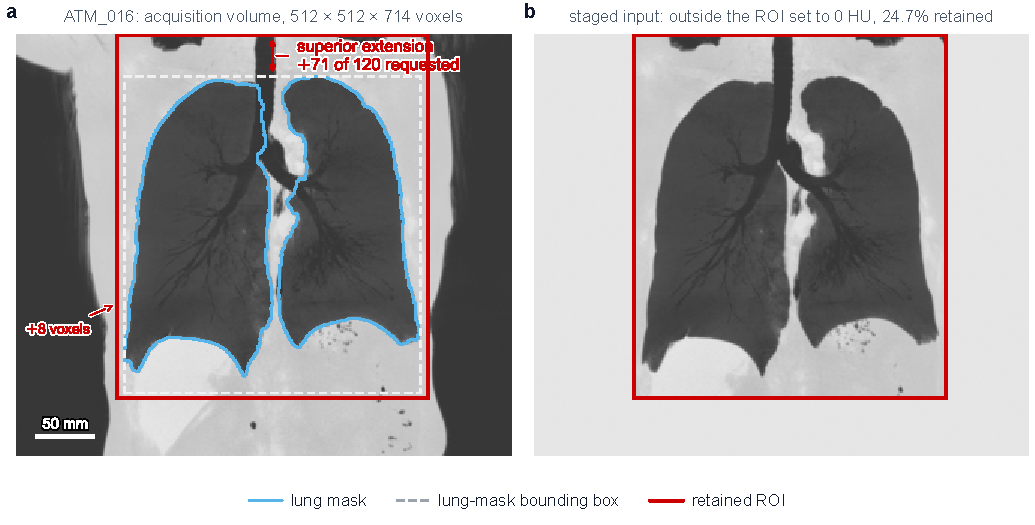
\includegraphics[width=\linewidth]{Figures/pdf/methods/lungroi/lung_roi_bbox.pdf}
  \caption[Airway region of interest]{The region of interest of Section~\ref{sec:pipeline} for
  ATM'22 case 016, coronal view. (a) Acquisition volume with the lung mask, its bounding box
  and the retained region. (b) The staged network input, with voxels outside the region set to
  $0$~HU; here $24.7\%$ of the volume is retained.}
  \label{fig:lung-roi}
\end{figure}

% ---------------------------------------------------------------------------
% ALTERNATIVE TO Figure~\ref{fig:lung-roi}, NOT AN ADDITION: the same staging drawn as a
% scene rather than as two coronal panels. Keep one, delete the other -- this block runs
% marker to marker. Drawn by dissertation/scripts/generate_lung_roi_3d_figure.py.
% ---------------------------------------------------------------------------
\begin{figure}[htbp]
  \centering
  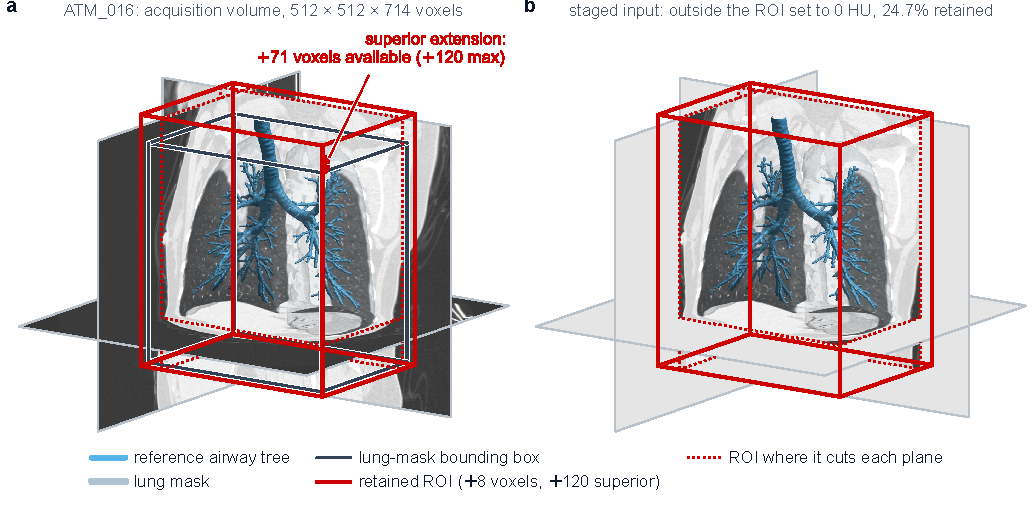
\includegraphics[width=\linewidth]{Figures/pdf/methods/lungroi/lung_roi_bbox_3d.pdf}
  \caption[Airway region of interest, three-dimensional]{The region of interest of
  Section~\ref{sec:pipeline} for ATM'22 case 016, seen from the patient's left and slightly
  above. Three orthogonal CT planes stand behind the anatomy, the lung mask is drawn as a
  translucent surface and the reference annotation as an isosurface; both boxes are drawn
  whole, in front of the scene, and dotted where the retained region cuts each plane. The
  solid box stands in front of the planes it is drawn over, so only the dotted rectangles
  meet the edge of the retained data. (a) Acquisition volume
  with the lung-mask bounding box and the retained region, whose superior face is raised to
  hold the cervical trachea; here the scan ends before the whole margin can be taken. (b)
  The staged network input, with voxels outside the region set to $0$~HU; here $24.7\%$ of
  the volume is retained. The airway tree is drawn for orientation only and takes no part
  in constructing the region, which is built from the lung mask alone. A coronal projection
  cannot show the anterior-posterior margin, which is two of the six faces.}
  \label{fig:lung-roi-3d}
\end{figure}
% ------------------------- end alternative figure --------------------------

\begin{table}[htbp]
  \centering
  \caption[nnU-Net configuration]{Planned and training configuration. Warm-started values apply
  to the Mean Teacher arms and the configuration-matched no-consistency continuation;
  supervised models use the from-scratch values.}
  \label{tab:nnunet-config}
  \begin{tabular}{ll}
    \toprule
    Setting & Value \\
    \midrule
    Configuration        & \texttt{3d\_fullres} \\
    Target spacing (mm)  & $0.820\times0.500\times0.820$ \\
    Patch size (voxels)  & $128\times160\times112$ \\
    Batch size           & 2 \\
    Normalisation        & \texttt{CTNormalization} (fingerprint percentiles) \\
    Optimiser            & SGD, Nesterov momentum 0.99, polynomial decay \\
    Learning rate        & $10^{-2}$ from scratch; $10^{-3}$ warm-started \\
    Schedule             & 1000 epochs from scratch; 500 warm-started, 250 iterations each \\
    Deep supervision     & disabled \\
    Mirroring            & disabled \\
    \bottomrule
  \end{tabular}
\end{table}

\begin{figure}[htbp]
  \centering
  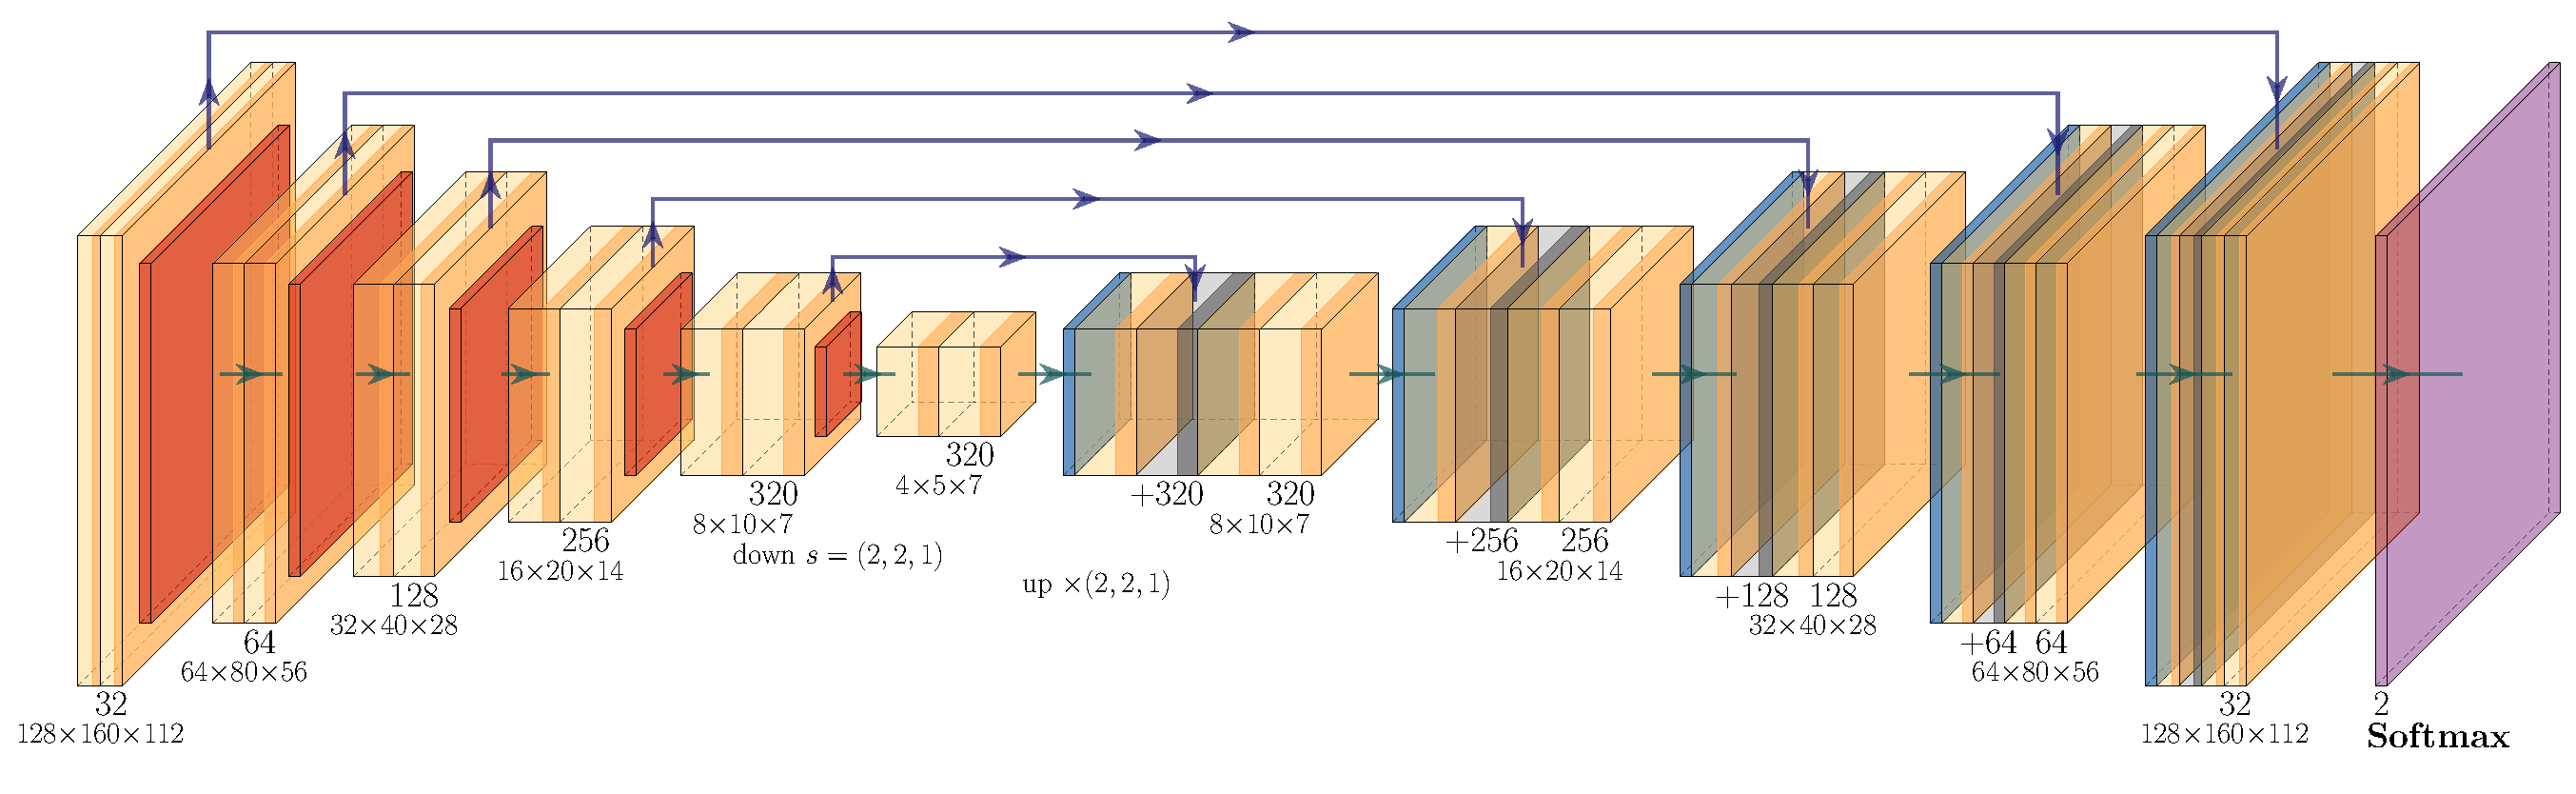
\includegraphics[width=\linewidth]{Figures/pdf/methods/mean_teacher/nnunet_backbone.pdf}
  \caption[Three-dimensional nnU-Net backbone]{The PlainConvUNet of
  Table~\ref{tab:nnunet-config}, shared by student and teacher. Block height and depth track
  spatial resolution and front-face width tracks channel count, with output channels and
  spatial size beneath each stage. Red slabs are strided convolutions, blue slabs transposed
  convolutions, and grey boxes the encoder features arriving on the skips. Drawn with
  PlotNeuralNet~\cite{iqbal2018plotneuralnet}.}
  \label{fig:nnunet-backbone}
\end{figure}

\section{Geometry-aware Mean Teacher}
\label{sec:mean-teacher}

\subsection{Notation and student--teacher formulation}

Let the labelled and unlabelled training sets be
\begin{equation}
  \mathcal{D}_{L}=\{(x_i,y_i)\}_{i=1}^{N_L},
  \qquad
  \mathcal{D}_{U}=\{x_j\}_{j=1}^{N_U},
  \label{eq:data}
\end{equation}
with $x$ a CT patch and $y\in\{0,1\}$ its airway annotation. Each step sampled one labelled and
one unlabelled patch. Writing $f_\theta$ for the airway probability channel of the softmax
output, the student with parameters $\theta_S$ and the teacher with parameters $\theta_T$ give
\begin{equation}
  p_{S,L}=f_{\theta_S}(\tilde{x}_L),
  \qquad
  p_{S,U}=f_{\theta_S}(\tilde{x}_U),
  \qquad
  p_{T,U}=f_{\theta_T}(x_U),
  \label{eq:predictions}
\end{equation}
where $\tilde{x}$ is the perturbed student view of Equation~\eqref{eq:perturbation}. The
teacher is not trained by back-propagation; its parameters are an exponential moving average of
the student's, updated after each optimiser step~\cite{tarvainen2017mean},
\begin{equation}
  \theta_T^{(t)}=\alpha_t\,\theta_T^{(t-1)}+(1-\alpha_t)\,\theta_S^{(t)},
  \qquad
  \alpha_t=\min\!\left(1-\frac{1}{t+1},\ \bar{\alpha}(e)\right),
  \label{eq:ema}
\end{equation}
with $t$ the step index and $e$ the epoch. Gradients flow only through the student, and the
final EMA teacher is the model used at inference. Figure~\ref{fig:mean-teacher-flow} shows the
resulting computation.

\begin{figure}[htbp]
  \centering
  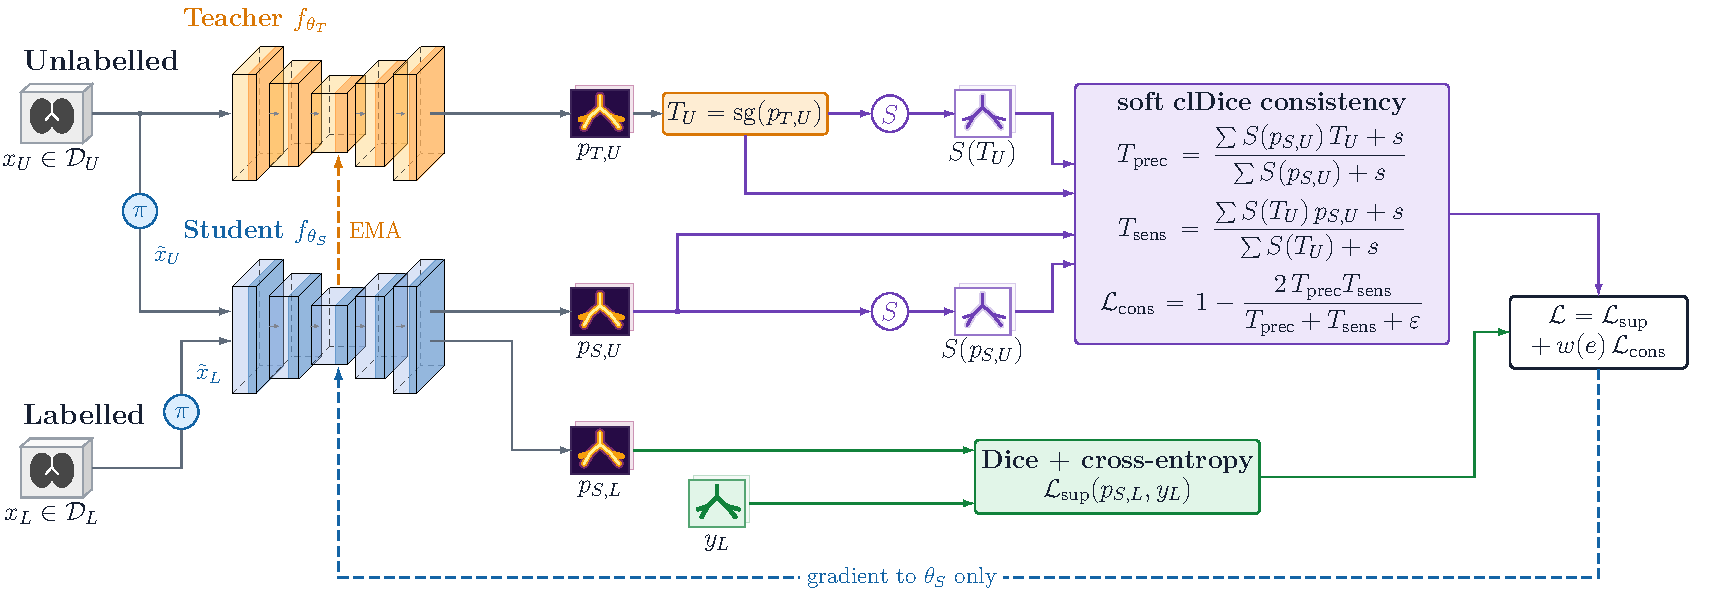
\includegraphics[width=\linewidth]{Figures/pdf/methods/mean_teacher/mean_teacher_flow.pdf}
  \caption[Two-stream Mean Teacher computation]{Two-stream Mean Teacher computation, with
  symbols as in Equations~\eqref{eq:data}--\eqref{eq:lcons}. Colour carries the roles: teacher
  warm, student blue, supervised path green and topology path purple, with back-propagation
  returning to the student alone along the dashed route. The image tiles are schematic rather
  than model outputs, and the network glyphs summarise the backbone of
  Figure~\ref{fig:nnunet-backbone}.}
  \label{fig:mean-teacher-flow}
\end{figure}

\subsection{Supervised objective}

The labelled stream uses nnU-Net's segmentation objective, the unweighted sum of soft Dice and
cross-entropy~\cite{isensee2021nnunet},
\begin{equation}
  \mathcal{L}_{\mathrm{sup}}(p,y)=\mathcal{L}_{\mathrm{Dice}}(p,y)+\mathcal{L}_{\mathrm{CE}}(p,y),
  \qquad
  \mathcal{L}_{\mathrm{Dice}}=1-\frac{2\sum_{\mathbf{u}}p(\mathbf{u})y(\mathbf{u})+\epsilon}
          {\sum_{\mathbf{u}}p(\mathbf{u})+\sum_{\mathbf{u}}y(\mathbf{u})+\epsilon},
  \label{eq:lsup}
\end{equation}
where $\mathbf{u}$ indexes voxels and $\epsilon$ is the framework's smoothing constant.

\subsection{Student perturbation}

The teacher receives the base view of an unlabelled patch and the student an additional
intensity perturbation,
\begin{equation}
  \tilde{x}=\pi(x)=a\,x+b+\eta,
  \qquad
  a\sim\mathcal{U}(1-s_a,\,1+s_a),
  \quad
  b\sim\mathcal{U}(-s_b,\,s_b),
  \quad
  \eta\sim\mathcal{N}(0,\sigma^2),
  \label{eq:perturbation}
\end{equation}
with $s_a=s_b=\sigma=0.1$, applied from epoch 5 to the student's whole input. Ordinary nnU-Net
augmentation is applied upstream and is therefore shared by both views, so the two outputs are
voxel-aligned and no inverse transform is required.

\subsection{Differentiable centreline extraction}

The consistency term compares centrelines, which requires a differentiable skeletonisation. The
implementation follows Shit et al.~\cite{shit2021cldice}, whose operators are the grey-scale
erosion and dilation of mathematical morphology under flat structuring
elements~\cite{serra1982morphology,haralick1987morphology,soille2003morphology}. Soft erosion
takes the minimum over a voxel and its six face-connected neighbours and soft dilation takes the
maximum over the full $3\times3\times3$ neighbourhood,
\begin{equation}
  \mathcal{E}(X)(\mathbf{u})=\!\!\min_{\mathbf{v}\in\mathcal{N}_6(\mathbf{u})\cup\{\mathbf{u}\}}\!\!X(\mathbf{v}),
  \qquad
  \mathcal{D}(X)(\mathbf{u})=\!\!\max_{\mathbf{v}\in\mathcal{N}_{26}(\mathbf{u})\cup\{\mathbf{u}\}}\!\!X(\mathbf{v}),
  \label{eq:morph}
\end{equation}
where $X$ is the input probability map, $\mathbf{u}$ denotes the voxel at which the operator
is evaluated, and $\mathbf{v}$ indexes voxels in its neighbourhood. 
$\mathcal{N}_6(\mathbf{u})$ and $\mathcal{N}_{26}(\mathbf{u})$ denote respectively the six
face-connected and the 26 surrounding neighbours of voxel $\mathbf{u}$.
Their composition $\mathcal{O}=\mathcal{D}\circ\mathcal{E}$ is the soft opening
of Shit et al.~\cite{shit2021cldice}. Ridge evidence at erosion depth $k$ is the positive part of what
the soft opening removes, an opening residual analogous to a white
top-hat~\cite{soille2003morphology}, and successive depths are combined by a differentiable
union,
\begin{align}
  X^{(0)}&=X,
  \qquad
  X^{(k)}=\mathcal{E}\!\left(X^{(k-1)}\right),
  \quad k=1,\dots,K,
  \nonumber\\
  \delta^{(k)}&=\operatorname{ReLU}\!\left(X^{(k)}-\mathcal{O}\!\left(X^{(k)}\right)\right),
  \quad k=0,\dots,K,
  \label{eq:residual}\\
  S^{(0)}&=\delta^{(0)},
  \qquad
  S^{(k)}=S^{(k-1)}+\operatorname{ReLU}\!\left(\delta^{(k)}-S^{(k-1)}\delta^{(k)}\right),
  \quad k=1,\dots,K.
  \label{eq:accumulate}
\end{align}
Residuals are therefore taken at depth $0$ and after each of $K=10$ erosion updates, and we
write $S(\cdot)=S^{(K)}$ for the resulting soft skeleton, illustrated in
Figure~\ref{fig:soft-skeleton-iteration} and set out procedurally in
Algorithm~\ref{alg:soft-skeleton}. Equations~\eqref{eq:residual} and~\eqref{eq:accumulate}
follow the form of Lantu\'ejoul's skeleton by
openings~\cite{lantuejoul1980skeleton,serra1982morphology}, with the set union over erosion
depths replaced by the probabilistic sum $a+b-ab$, the standard fractional union that keeps the
accumulation differentiable~\cite{klir1995fuzzy,bloch1995fuzzymorphology}.

\begin{figure}[htbp]
  \centering
  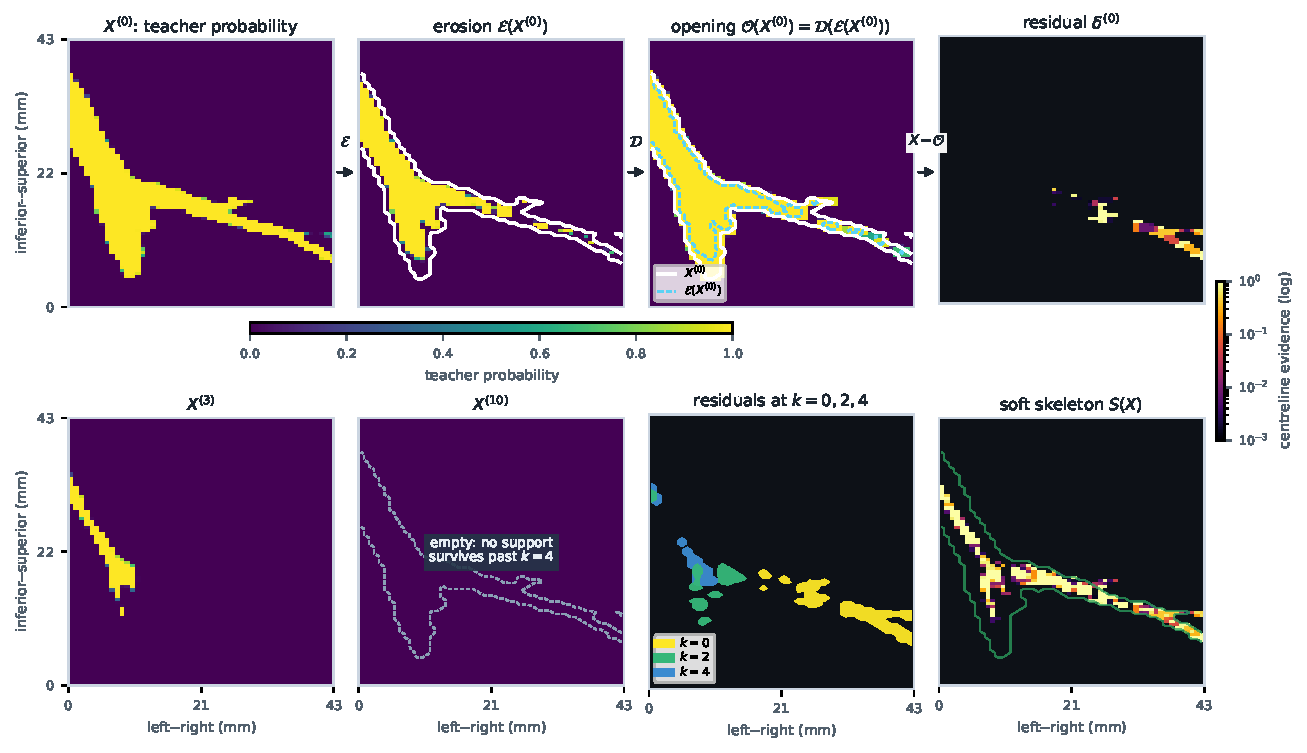
\includegraphics[width=\linewidth]{Figures/pdf/methods/cldice/soft_skeleton_iteration.pdf}
  \caption[Differentiable soft skeletonisation]{Equations~\eqref{eq:morph}--\eqref{eq:accumulate}
  on a real EMA-teacher airway-probability patch, as a maximum projection through a seven-voxel
  coronal slab. Top row, one iteration: erosion, the opening $\mathcal{O}(X^{(0)})$, and the
  residual $\delta^{(0)}$. Contours give $X^{(0)}$ at $0.5$ (solid white) and where erosion left
  it (dashed cyan), so the trunk is regrown by the dilation and the thin distal branch is not.
  Bottom row, successive erosion depths and their union, the soft skeleton $S(X)$; the grey
  dashed outline marks the original airway support. Green is the reference airway, for
  orientation only.}
  \label{fig:soft-skeleton-iteration}
\end{figure}

An implementation-matched diagnostic quantified how this finite operator allocated its mass.
Six foreground-centred, training-shaped patches were sampled from each of four final EMA-teacher
probability maps. Teacher foreground and $S(T_U)$ were assigned to the operational calibre of the
nearest reference centreline voxel, and their mass shares were aggregated over the 24 patches.
The calculation was repeated after twofold trilinear upsampling, using $K=20$ to preserve the
physical erosion range, and timed with gradient checkpointing. This probe characterises the
implemented loss on fitted predictions; it is not a training arm or an estimate of the Mean
Teacher effect.

\subsection{Geometry-aware consistency}
\label{sec:consistency}

The consistency target is the detached teacher probability map,
$T_U=\operatorname{sg}(p_{T,U})$, where $\operatorname{sg}$ denotes the stop-gradient. Student
and target are compared by the topology precision and topology sensitivity of Shit et
al.~\cite{shit2021cldice},
\begin{equation}
  T_{\mathrm{prec}}
  =\frac{\sum_{\mathbf{u}}S(p_{S,U})T_U+s}{\sum_{\mathbf{u}}S(p_{S,U})+s},
  \qquad
  T_{\mathrm{sens}}
  =\frac{\sum_{\mathbf{u}}S(T_U)\,p_{S,U}+s}{\sum_{\mathbf{u}}S(T_U)+s},
  \label{eq:tterms}
\end{equation}
with smoothing $s=1$ in numerator and denominator, and the consistency loss is one minus their
harmonic mean,
\begin{equation}
  \mathcal{L}_{\mathrm{cons}}
  =1-\frac{2\,T_{\mathrm{prec}}T_{\mathrm{sens}}}{T_{\mathrm{prec}}+T_{\mathrm{sens}}},
  \label{eq:lcons}
\end{equation}
which is soft clDice~\cite{shit2021cldice}, here evaluated between the student and the EMA
teacher rather than between a prediction and an annotation. Both terms are computed per sample
and averaged over the batch.

The voxel-MSE arm replaces Equation~\eqref{eq:lcons} with the squared-error consistency of
Tarvainen and Valpola~\cite{tarvainen2017mean}, applied per voxel to the airway channel as in
semi-supervised 3D segmentation~\cite{yu2019uamt},
\begin{equation}
  \mathcal{L}_{\mathrm{MSE}}
  =\frac{1}{|\Omega|}\sum_{\mathbf{u}\in\Omega}
   \left(p_{S,U}(\mathbf{u})-T_U(\mathbf{u})\right)^{2},
  \label{eq:lmse}
\end{equation}
over the patch domain $\Omega$, with every other setting held fixed.

Wallace and Dahabreh define separate class-specific Brier scores~\cite{wallace2014imbalanced};
Bellinger et al. average these to form the balanced Brier score~\cite{bellinger2020remix}.
Adapting this to soft teacher targets, voxels were split into teacher-predicted foreground
($\geq0.5$) and background ($<0.5$). For non-empty groups,
\begin{equation}
  \begin{aligned}
    \mathrm{MSE}_{\mathrm{fg}}
    &=\frac{1}{N_{\mathrm{fg}}}
      \sum_{\substack{\mathbf{u}\in\Omega\\T_U(\mathbf{u})\geq0.5}}
      \left(p_{S,U}(\mathbf{u})-T_U(\mathbf{u})\right)^2,\\
    \mathrm{MSE}_{\mathrm{bg}}
    &=\frac{1}{N_{\mathrm{bg}}}
      \sum_{\substack{\mathbf{u}\in\Omega\\T_U(\mathbf{u})<0.5}}
      \left(p_{S,U}(\mathbf{u})-T_U(\mathbf{u})\right)^2,\\
    \mathcal{L}_{\mathrm{balMSE}}
    &=\frac{1}{2}\left(\mathrm{MSE}_{\mathrm{fg}}+\mathrm{MSE}_{\mathrm{bg}}\right),
  \end{aligned}
  \label{eq:lbalancedmse}
\end{equation}
where $N_{\mathrm{fg}}$ and $N_{\mathrm{bg}}$ are the respective voxel counts; an empty
group contributed zero. This gives each predicted group equal weight without centreline geometry.

\subsection{Training objective and schedule}

The total objective is the supervised loss plus a ramped consistency term,
\begin{equation}
  \mathcal{L}=\mathcal{L}_{\mathrm{sup}}\!\left(p_{S,L},y_L\right)
  +w(e)\,\mathcal{L}_{\mathrm{cons}}\!\left(p_{S,U},T_U\right),
  \label{eq:total}
\end{equation}
with the Gaussian ramp of Laine and Aila~\cite{laine2017temporal},
\begin{equation}
  w(e)=w_{\max}\exp\!\left[-5\left(1-r(e)\right)^{2}\right],
  \qquad
  r(e)=\operatorname{clamp}\!\left(\frac{e-e_0}{e_r},\,0,\,1\right),
  \label{eq:ramp}
\end{equation}
and $w(e)=0$ for $e<e_0$. Following UA-MT~\cite{yu2019uamt} we set $w_{\max}=0.1$, with warm-up
$e_0=5$ epochs and ramp $e_r=20$ epochs. The EMA ceiling $\bar{\alpha}$ of
Equation~\eqref{eq:ema} is $0.99$ during the ramp and $0.999$
afterwards~\cite{tarvainen2017mean}. Warm-started training ran for 500 epochs at initial
learning rate $10^{-3}$, following nnU-Net's fine-tuning
guidance~\cite{nnunetdocs_finetuning,wald2024maepretraining}; each Mean Teacher fold was
warm-started from its same-numbered supervised checkpoint.

\section{Experimental design}
\label{sec:experimental-design}

Continuation arms used 16 labelled training cases, four internal-validation cases and 240
label-withheld cases, with a common crop, architecture, sampler, schedule and final EMA
deployment. The primary contrast was
\begin{equation}
  \mathcal{L}_{\mathrm{control}}=\mathcal{L}_{\mathrm{sup}},
  \qquad
  \mathcal{L}_{\mathrm{MT}}=\mathcal{L}_{\mathrm{sup}}+w(e)\,\mathcal{L}_{\mathrm{cons}}.
  \label{eq:contrast}
\end{equation}
The control omitted the unlabelled gradient and teacher forward pass.

\ifshowcurrentcontrol
\begin{currentcontrolroute}
\noindent\textbf{Current fitted-checkpoint route.}
The scored control and Mean Teacher runs named the same supervised warm start, but transfer
excluded their segmentation heads and their RNG, augmentation and CUDA trajectories were
independent. They therefore provide a single-run configuration contrast, not a realised-paired
control.
\end{currentcontrolroute}
\fi

\ifshowpairedcontrol
\begin{pairedcontrolroute}
\noindent\textbf{Prospective paired-seed route.}
Five fold~0 control--Mean Teacher pairs load the same complete checkpoint within each pair and
share the seeded data order, augmentation draws and deterministic CUDA settings. Only pairs in
which both arms finish are analysed; three complete pairs are the minimum.
\end{pairedcontrolroute}
\fi

Plain and class-balanced voxel MSE, consistency weight and skeleton depth are ablations; the
five-fold Mean Teacher ensemble and 110-case supervised model provide deployment and scale
context, respectively.

\begin{table}[htbp]
  \centering
  \small
  \setlength{\tabcolsep}{3pt}
  \caption[Experimental arms and their scientific roles]{Experimental arms retained in the
  main study. ``L'' and ``U'' denote labelled and label-withheld training cases.}
  \label{tab:experimental-arms}
  \begin{tabular}{@{}>{\raggedright\arraybackslash}p{0.16\linewidth}
                      >{\raggedright\arraybackslash}p{0.25\linewidth}
                      >{\raggedright\arraybackslash}p{0.13\linewidth}
                      >{\raggedright\arraybackslash}p{0.36\linewidth}@{}}
    \toprule
    Role & Arm & Training data & Question answered \\
    \midrule
    \ifshowcurrentcontrol
    \textcolor{ImperialBlue}{Current contrast} & \textcolor{ImperialBlue}{Control and soft-clDice MT} & \textcolor{ImperialBlue}{16 L $+$ 240 U} & \textcolor{ImperialBlue}{Available fitted-checkpoint comparison} \\
    \fi
    \ifshowpairedcontrol
    \textcolor{ImpRed}{Seeded contrast} & \textcolor{ImpRed}{Five control--soft-clDice pairs} & \textcolor{ImpRed}{16 L $+$ 240 U} & \textcolor{ImpRed}{Training-run variation at fixed fold} \\
    \fi
    Objectives & Plain and balanced voxel MSE & 16 L $+$ 240 U & Geometry versus voxel agreement \\
    Parameters & Soft-clDice weight and skeleton depth & 16 L $+$ 240 U & Sensitivity around the primary setting \\
    Deployment & Five-fold soft-clDice ensemble & 16 L/fold $+$ 240 U & Absolute ensemble performance \\
    References & 16-label seed; 110-case supervised model & 16 L; 88 L & Warm-start and label-scale context \\
    \bottomrule
  \end{tabular}
\end{table}

\section{Inference and post-processing}

Predictions used nnU-Net's sliding-window inference without test-time augmentation, and the
native argmax output is the primary result; no probability threshold was tuned. For Mean
Teacher arms the final EMA teacher is the model evaluated. A single connected-component
sensitivity analysis is reported alongside, retaining the six-connected component that
intersects an affine-derived window covering the superior quarter and the central half of each
remaining axis, and falling back to the largest component if none intersects. Checkpoint
provenance is given in Appendix~\ref{AppendixA}.

\section{Evaluation protocol and tree analysis}
\label{sec:evaluation}

\subsection{Voxel-level and topology-aware metrics}

Let $P$ be the predicted foreground and $G$ the reference airway mask, with
\begin{equation}
  \operatorname{Dice}=\frac{2|P\cap G|}{|P|+|G|},
  \qquad
  \operatorname{Prec}=\frac{|P\cap G|}{|P|},
  \qquad
  \operatorname{Rec}=\frac{|P\cap G|}{|G|}.
  \label{eq:voxel}
\end{equation}
Following the ATM'22 protocol the reference is reduced to its largest connected component
before skeletonisation, which uses three-dimensional medial-axis thinning~\cite{lee1994thinning}. Writing $S_G$ for that skeleton and $S_P$ for the skeleton of the
prediction, tree-length detected and topology precision are
\begin{equation}
  \operatorname{TLD}=\frac{|S_G\cap P|}{|S_G|},
  \qquad
  \operatorname{TPrec}=\frac{|S_P\cap G|}{|S_P|}.
  \label{eq:tld}
\end{equation}
Branch detection parses $S_G$ into branches by removing junction
voxels and discarding fragments shorter than five voxels; for reference branch $b$ with
skeleton $S_b$,
\begin{equation}
  c_b=\frac{|S_b\cap P|}{|S_b|},
  \qquad
  \operatorname{BD}=\frac{1}{N_B}\sum_{b=1}^{N_B}\mathbf{1}\!\left[c_b\ge0.8\right].
  \label{eq:bd}
\end{equation}
Dice, voxel precision, TLD and BD are the four primary measures. Where reported, the secondary
ATM-style clDice quantity is the harmonic mean
$2\,\operatorname{TLD}\operatorname{TPrec}/
(\operatorname{TLD}+\operatorname{TPrec})$. Because its TLD term uses the largest connected
component of the reference while its topology-precision term uses the full prediction, this is
a mixed-support diagnostic rather than standard full-mask clDice. All metrics are computed per
patient and reported as macro means over cases.

\subsection{Calibre-stratified recovery}
\label{sec:methods-calibre}

Recovery was stratified by local airway calibre, defined granulometrically as what a voxel fits
inside~\cite{matheron1975randomsets,serra1982morphology}. The operational calibre uses the
operators of Equation~\eqref{eq:morph}, so that it speaks about what the training objective can
resolve,
\begin{equation}
  n(\mathbf{u})=\max\left\{n:\ \mathbf{u}\in\mathcal{D}^{\,n}\!\left(\mathcal{E}^{\,n}(G)\right)\right\},
  \label{eq:opclass}
\end{equation}
where class $n$ corresponds to a thickness of $\{2n+1,2n+2\}$ voxels, so that the histogram of
$n$ over the reference tree is an opening size distribution, or pattern
spectrum~\cite{maragos1989patternspectrum,soille2003morphology}.
Intuitively, $n(\mathbf{u})$ is the largest erosion--dilation scale that the airway
surrounding $\mathbf{u}$ survives; larger values therefore correspond to locally thicker
airways.

The anatomical calibre is the Euclidean local thickness in millimetres, the diameter of the
largest ball that fits inside the structure and contains the
voxel~\cite{hildebrand1997thickness,dougherty2007localthickness},
\begin{equation}
  \tau(\mathbf{u})=2\max\left\{r:\ \mathbf{u}\in\mathcal{O}_{r}(G)\right\},
  \label{eq:mmthickness}
\end{equation}
with $\mathcal{O}_r$ opening by a ball of radius $r$ on the voxel spacing. Both refer to lumen
calibre, not airway-wall thickness.

Writing $S_G^{(k)}$ for the reference centreline voxels in
band $B_k$ under either definition, band-wise recovery is
\begin{equation}
  \operatorname{TLD}_k=\frac{\left|S_G^{(k)}\cap P\right|}{\left|S_G^{(k)}\right|}.
  \label{eq:tldband}
\end{equation}
Calibre is defined from the reference tree and the same banding is applied to every arm.

\subsection{Branch-depth analysis}
\label{sec:methods-depth}

Branch depth was used as a measure of position within the airway tree, following the
established practice of reducing a segmented tree to its centreline and analysing it branch by
branch~\cite{tschirren2005airway,palagyi2006airway}. The reference
skeleton was first divided into branches as in Equation~\eqref{eq:bd}, and these branches
were connected to form a graph. The ATM'22 branch-refinement procedure was then applied
iteratively until the graph no longer changed. In particular, consecutive branch fragments
connected through only a single child were absorbed into the same path, so that depth
increased at branch divisions rather than at every skeleton fragment.

On the resulting branch graph $G_B=(V_B,E_B)$, each node $v\in V_B$ represents a refined
airway branch and each edge represents a connection between branches. The largest-volume
branch was taken as the graph root; in practice this corresponded to the tracheal branch
in the reference trees examined,
\begin{equation}
  v_0=\operatorname*{arg\,max}_{v\in V_B}\operatorname{Vol}(v),
\end{equation}
and the depth of branch $v$ was defined as its graph distance from this root,
\begin{equation}
  d(v)=\operatorname{dist}_{G_B}(v_0,v).
  \label{eq:depth}
\end{equation}

Thus, $d(v)$ approximately counts the number of successive branch divisions separating a
branch from the trachea. It is therefore treated as a branching-order proxy
rather than as an anatomical Weibel generation~\cite{weibel1963morphometry}, which is fixed by
anatomical correspondence rather than by distance on a parsed
graph~\cite{tschirren2005airway}.

Figure~\ref{fig:branch-depth-definition} shows this assignment on an example reference tree
together with the distribution of annotated centreline length over depth across all 260
training cases. Reference centreline length is concentrated around intermediate depths,
peaking at depth six, and the external validation cohort follows the same distribution to
within 2.3 percentage points at every depth. Airway trees do not all end at the same
generation: the shallowest validation tree ends at depth eight, and only 46 of the 260 training
cases reach depth twelve. Depth-stratified recovery is therefore reported over depths zero to
seven individually, with depths eight and above pooled as $8+$, which keeps all 20 cases in
every point and retains the deep tree rather than discarding it.

\begin{figure}[htbp]
  \centering
  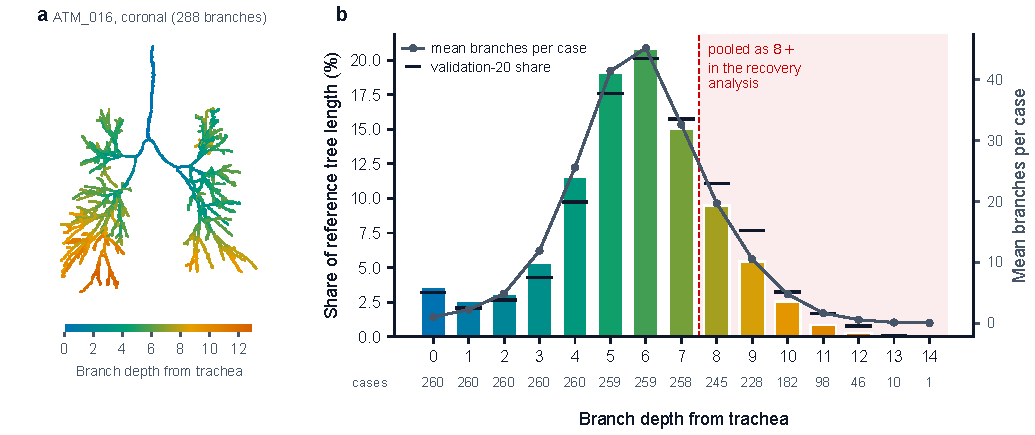
\includegraphics[width=\linewidth]{Figures/pdf/methods/depth/branch_depth_definition.pdf}
  \caption[Branch-depth coordinate and cohort distribution]{The branch-depth coordinate of
  Equation~\eqref{eq:depth}. (a) Coronal projection of the ATM\_016 reference skeleton, each
  centreline voxel coloured by the depth of its refined branch; the patient's right is on the
  left. (b) Share of annotated centreline length at each depth over the 260 training cases
  (bars, left axis), mean refined branches per case (line, right axis), and the corresponding
  share in the 20-case external validation cohort (black dashes). The row beneath the axis
  gives how many cases reach each depth. Shading marks the depths pooled into the $8+$ bin of
  the depth-stratified results.}
  \label{fig:branch-depth-definition}
\end{figure}

For a depth group $D_k$, the corresponding reference centreline is
\begin{equation}
  S_G^{(k)}
  =
  \bigcup_{v:\,d(v)\in D_k} S_v,
\end{equation}
and recovery within that group is calculated using the band-wise TLD definition of
Equation~\eqref{eq:tldband}. Depth labels are derived only from the reference tree and are
applied identically to every model.

\paragraph{Statistical comparisons.}
The patient is the unit of evaluation and checkpoint comparisons are paired because every arm
segments the same cases. Per-patient arm-minus-comparator differences are summarised by their
mean, the number favouring the arm, a pointwise 95\% paired-$t$ interval and the standardised
effect $d_z$; figures explicitly labelled as bootstrap intervals instead resample patients as
pairs. Two-sided paired $t$-tests are accompanied by Wilcoxon signed-rank tests, with
Bonferroni correction within each contrast across Dice, voxel precision, TLD, BD and the
secondary ATM-style clDice diagnostic. These patient-level intervals condition on the fitted
checkpoints and do not estimate training-run variation. For the prospective replication, a
cohort-mean treatment effect is first calculated within each complete seed pair and the
resulting replicate-level effects are reported by their mean, standard deviation and range;
patients from different training replicates are not treated as independent observations.

\section{Reproducibility}

Exact case identifiers, per-arm memberships, fold assignments, configuration files, training
commands and checkpoint provenance are provided in Appendix~\ref{AppendixA}. Training used
non-deterministic CUDA operations and mixed precision, and each experimental configuration was
trained once, so results are reproducible as a configuration rather than bitwise.
